\documentclass[11pt]{article} % 
\usepackage[pdftex]{graphicx}
\usepackage{fullpage}
\usepackage{graphicx}
\usepackage{graphics}
\usepackage{psfrag}
\usepackage{pgf}
\usepackage{color}
\usepackage{tikz}
\usetikzlibrary{arrows,automata}
\usepackage[latin1]{inputenc}
\usepackage{amsthm}
\usepackage{amsmath,amssymb}
\usepackage{enumerate}
\setlength{\textwidth}{6.5in}
\setlength{\textheight}{9in}
\newcommand{\N}{\mathbb{N}}
\newcommand{\Z}{\mathbb{Z}}
\newcommand{\R}{\mathbb{R}}
\newcommand{\Q}{\mathbb{Q}}
\newcommand{\C}{\mathbb{C}}
\newcommand{\PP}{\mathbb{P}}
\newcommand{\tab}{\;\;\;\;\;}
\newcommand{\inv}{^{-1}}
\newcommand{\tr}{\textrm}
\newcommand{\lc}{\sqcup}

\begin{document}

\hfill Robert Johns

\hfill January 23, 2014

\begin{center} {\Large CSCI 678: Statistical Analysis of Simulation Models}\\{\large Homework 1}\end{center}

\begin{enumerate}

%1
\item Modify the program \texttt{buffon.c} to allow for 100, 1000, 10000, 100000 and 1000000 replications and make a plot of the sample size versus the estimated probability of crossing.  Indicate the theoretical value on the graph and run the program five times as above.

{\bf Solution:} The resulting graph follows:

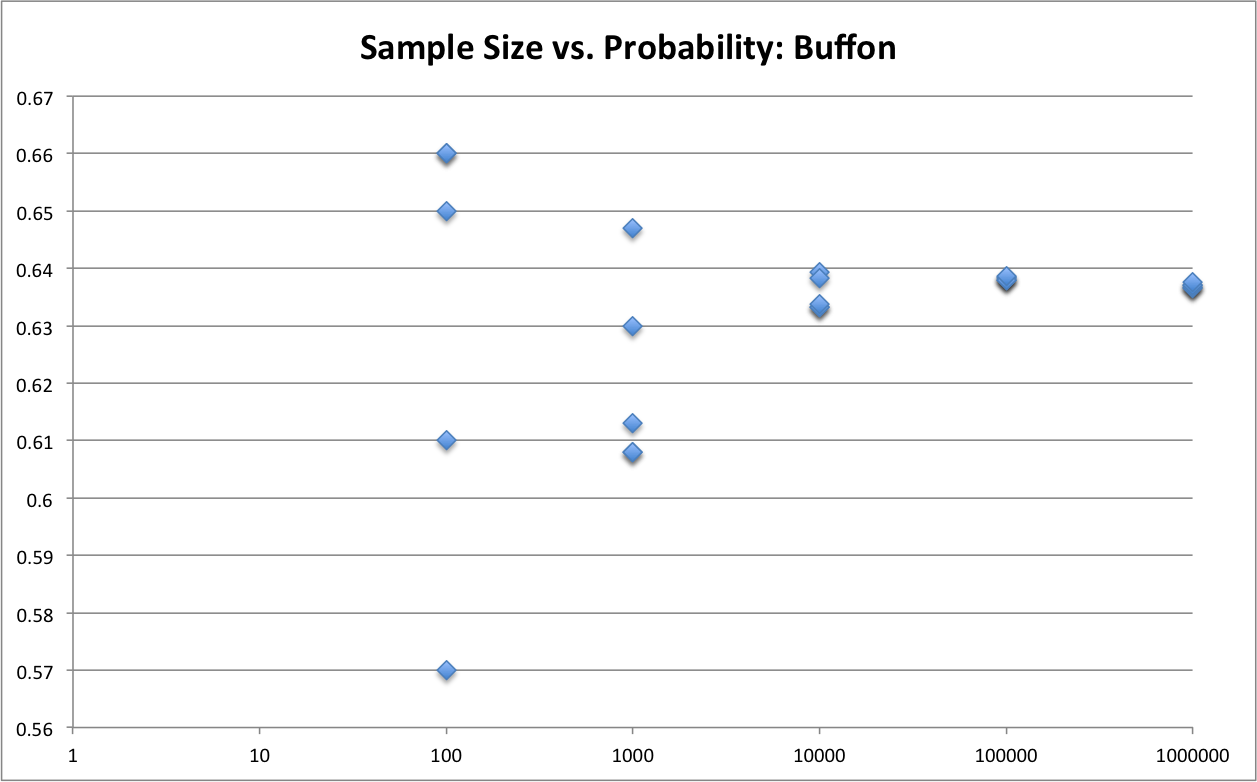
\includegraphics[scale = 0.65]{asm1.png}

%2
\item Generate a similar result for the program \texttt{craps.c}.  Include a horizontal line that gives the true probability of winning at Craps, which is 244/495.  

{\bf Solution} The resulting graph follows

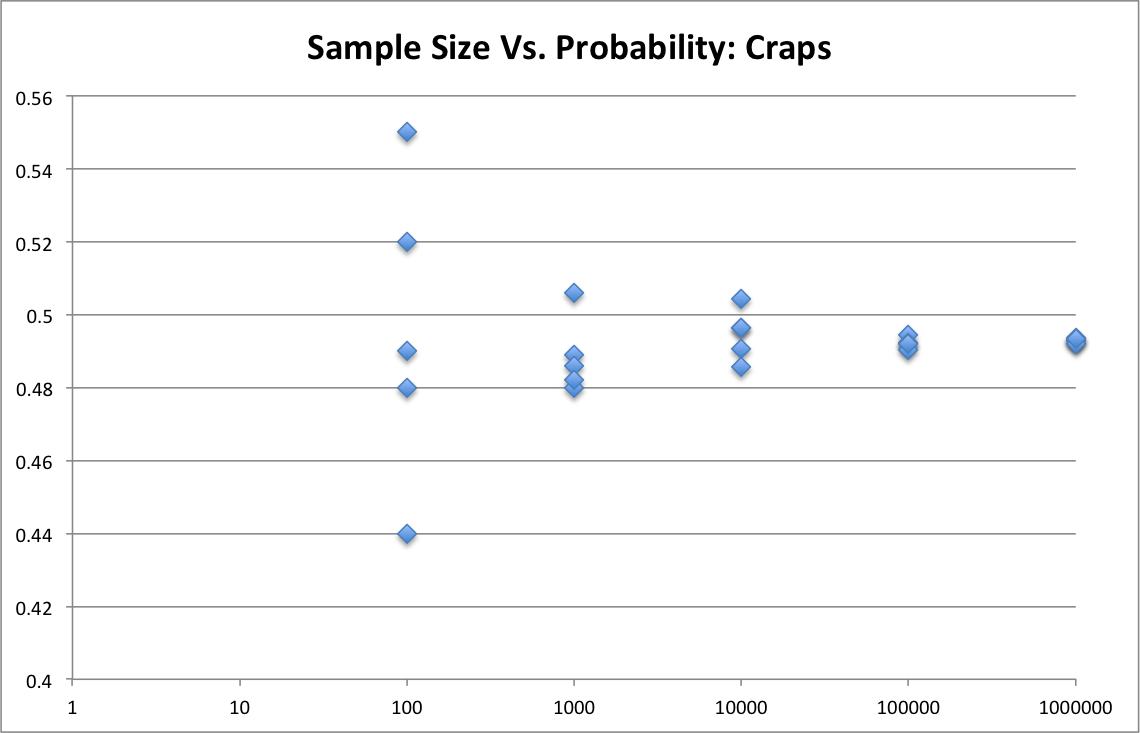
\includegraphics[scale = .6]{asm2.png}

%3
\item The following questions concern the program \texttt{ssq3.c}.

\begin{enumerate}

%3a
\item What are the two distinct types of event in this simulation?

{\bf Solution:} A job's arrival into the service node, and a completion of service for a job, which serves as a departure from the node.

%3b
\item What variable name is used for the simulation clock?

{\bf Solution:} The variable \texttt{current} in the structure \texttt{t} saves the clock time (so \texttt{t.current} is the full reference).

%3c
\item What variable/data structure name is used for the calendar (future event list)?

{\bf Solution:} The structure \texttt{t} is used to store the current time (\texttt{t.current}), the time of the next event to happen (\texttt{t.next}), the last arrival time (\texttt{t.last}) and the next scheduled events of both types (\texttt{t.arrival} and \texttt{t.completion}).  The \texttt{t} data structure, a ``\texttt{struct}" (essentially a class without methods in C), store all these event times, which make up the calendar of the next-event simulation.

%3d
\item Modify \texttt{ssq3.c} to print the minimum, median and maximum wait times in the service node, in addition to the variables already printed.  Comment on the values you obtain with your new code.  Make specific reference to the difference to the difference between the average and median waits in the service node.

{\bf Solution:} See attached code (\texttt{ssq3.c}).  The program produces the following output:

\begin{verbatim}for 10025 jobs
   average interarrival time =   1.99
   average wait ............ =   3.92
   average delay ........... =   2.41
   average service time .... =   1.50
   average # in the node ... =   1.96
   average # in the queue .. =   1.21
   utilization ............. =   0.75
   minimum wait time ....... =   1.000149
   median wait time ........ =   3.040863
   maximum wait time ....... =   24.564435\end{verbatim}
   
 We see that the average wait is roughly 0.88 seconds greater than the median wait.  This makes sense, because there will never be a wait less than 0 (in fact, 1 is the minimum) but a wait can theoretically be infinite, and the maximum 24.56 seconds, so the larger outliers will bring the average up more than the smaller outliers bring it down.  The disparity between the mean and median tells us that there are more jobs with wait times less than the mean than there are jobs with service times greater than the mean, which follows from the explanation above.

\end{enumerate}

\end{enumerate}

\end{document}